In this section we will discuss the different methods required to effectively run classical computational simulations of the protocols described in Section \ref{section:protocols} such that, for any choice of qubit pure states and rank-1 POVMs, the quantum predictions in Equation (\ref{eq:prob_quantum}) are reproduced classically following Equation (\ref{eq:prob_classic}), i.e.
\begin{equation}
\forall \rho, \{B_{k}\}:\quad tr(\rho B_{k}) = \int_{\lambda} d\lambda\ \pi(\lambda) \sum_{c=1}^{d_C} p_A(c|\rho, \lambda)\ p_B(k|\{B_{k}\}, c, \lambda)    
\end{equation}
and for a Bell singlet state $\ket{\Psi^{-}}$ and any choice of PVMs, the quantum predictions in Equation (\ref{eq:prob_quantum_bell}) are reproduced classically following Equation (\ref{eq:prob_classic_bell}), i.e.
\begin{equation}
\forall A_{x}, B_{y}: |\bra{\Psi_{ij}}\ket{a_{x}} \otimes \ket{b_{y}}|^{2} = \int_{\lambda} d\lambda\ \pi(\lambda) p_A(c|A_{x}, \lambda)\ p_B(b_{y}|B_{y}, c, \lambda)
\end{equation}


The main goal is to carry out these simulations using standard classical computations, but some particular results will be confronted with the outcomes from quantum circuit simulators and quantum computers, therefore there will be specific subsections devoted to the implementation of generalized measurements in a quantum circuit model. 
\subsection{State preparation}
In the classical simulations, the state preparation would require to produce a random qubit pure state first, and then to compute the corresponding Bloch vector to be used later by Alice. 

In the prepare-and-measure scenario, Alice uses the Bloch vector representation of the qubit's pure state, and Bob's POVMs,  proportional to rank-1 projectors, are expressed as the outer product of the associated Bloch vectors. In the Bell scenario, Alice also uses the Bloch vector corresponding to the local projective measurement projectors. In addition, in all these protocols, Alice and Bob share two random normalized vectors $\vec{\lambda}_1, \vec{\lambda}_2 \in \mathbb{R}^{3}$, which must be uniformly and independently distributed on the unit sphere $S_2$, which is analogous to generate random Bloch vectors in the Bloch sphere. Given the fact that the classical probabilities obtained with the different protocols must be equivalent to the quantum probabilities for any state and POVM measure, and that generating a true shared randomness is a fundamental element of the classical protocols, it is of key importance to be able prepare random normalized vectors uniformly distributed along the unit radius sphere $S_2$. Hence, the randomized qubit state preparation in the form of Bloch vectors is not only the building block for the state preparation itself, but plays also a critical role in the measurement construction and the shared randomness creation.

To produce a random qubit pure state we should obtain a random unitary matrix and then apply the unitary transformation to the zero qubit state, resembling the time evolution of a qubit from a zero initial state. The random unitary matrix can be generated by just building a matrix of normally distributed complex numbers, and then apply the Gram-Schmidt QR decomposition to orthogonalize the matrix, see \cite{ozols2009}, \cite{zyczkowski1994}. 

The resulting random qubit state distribution can be validated using the corresponding Bloch vector distribution along the unit radius sphere. A tessellation scheme called HEALPix \cite{healpix}, which produces a hierarchical and equal-area iso-latitude pixelation of a sphere, could be used to show that the random Bloch vectors are uniformly and independently distributed in the Bloch sphere. Given that each pixel in HEALPix covers the same surface area as every other pixel (see Figure \ref{fig:healpix_sphere}), we can group the Bloch vector distribution along the different pixel indices (see Figure \ref{fig:healpix_numbering}), and check whether the resulting distribution is uniform as expected.

\begin{figure}[!ht]
\begin{center}
\centerline{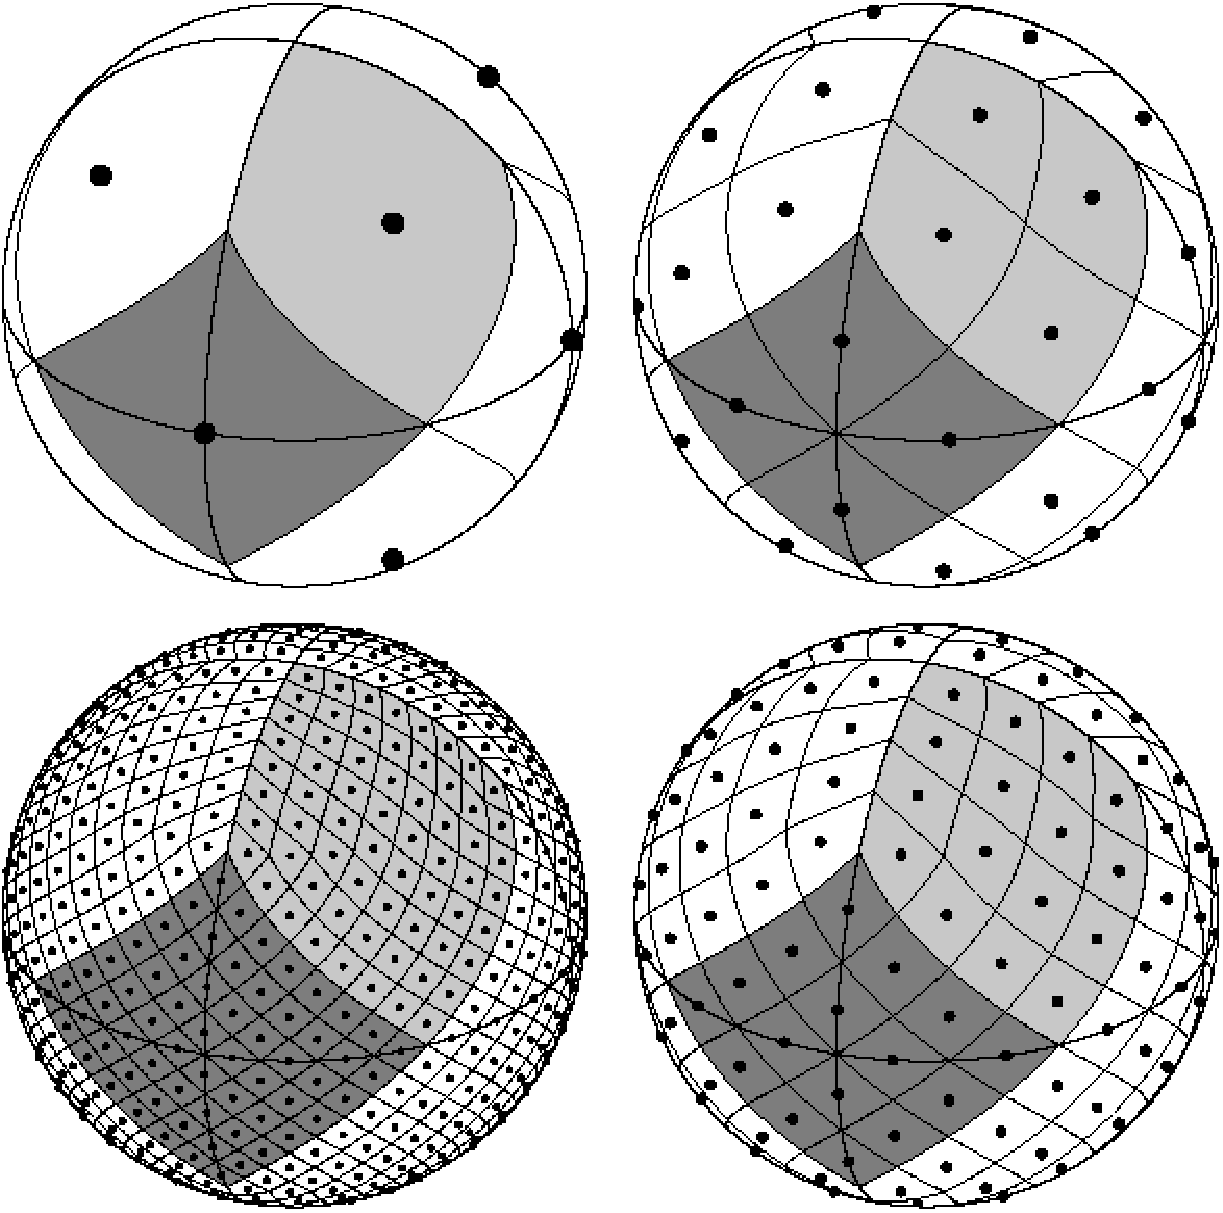
\includegraphics[height=5.5cm]{images/healpix4.pdf}}
\caption[Orthographic view of Healpix partition of the sphere]%
{\label{fig:healpix_sphere}%
Orthographic view of HEALPix partition of the sphere.}
\end{center}
\end{figure}

\begin{figure} [!ht]
\begin{center}
\centerline{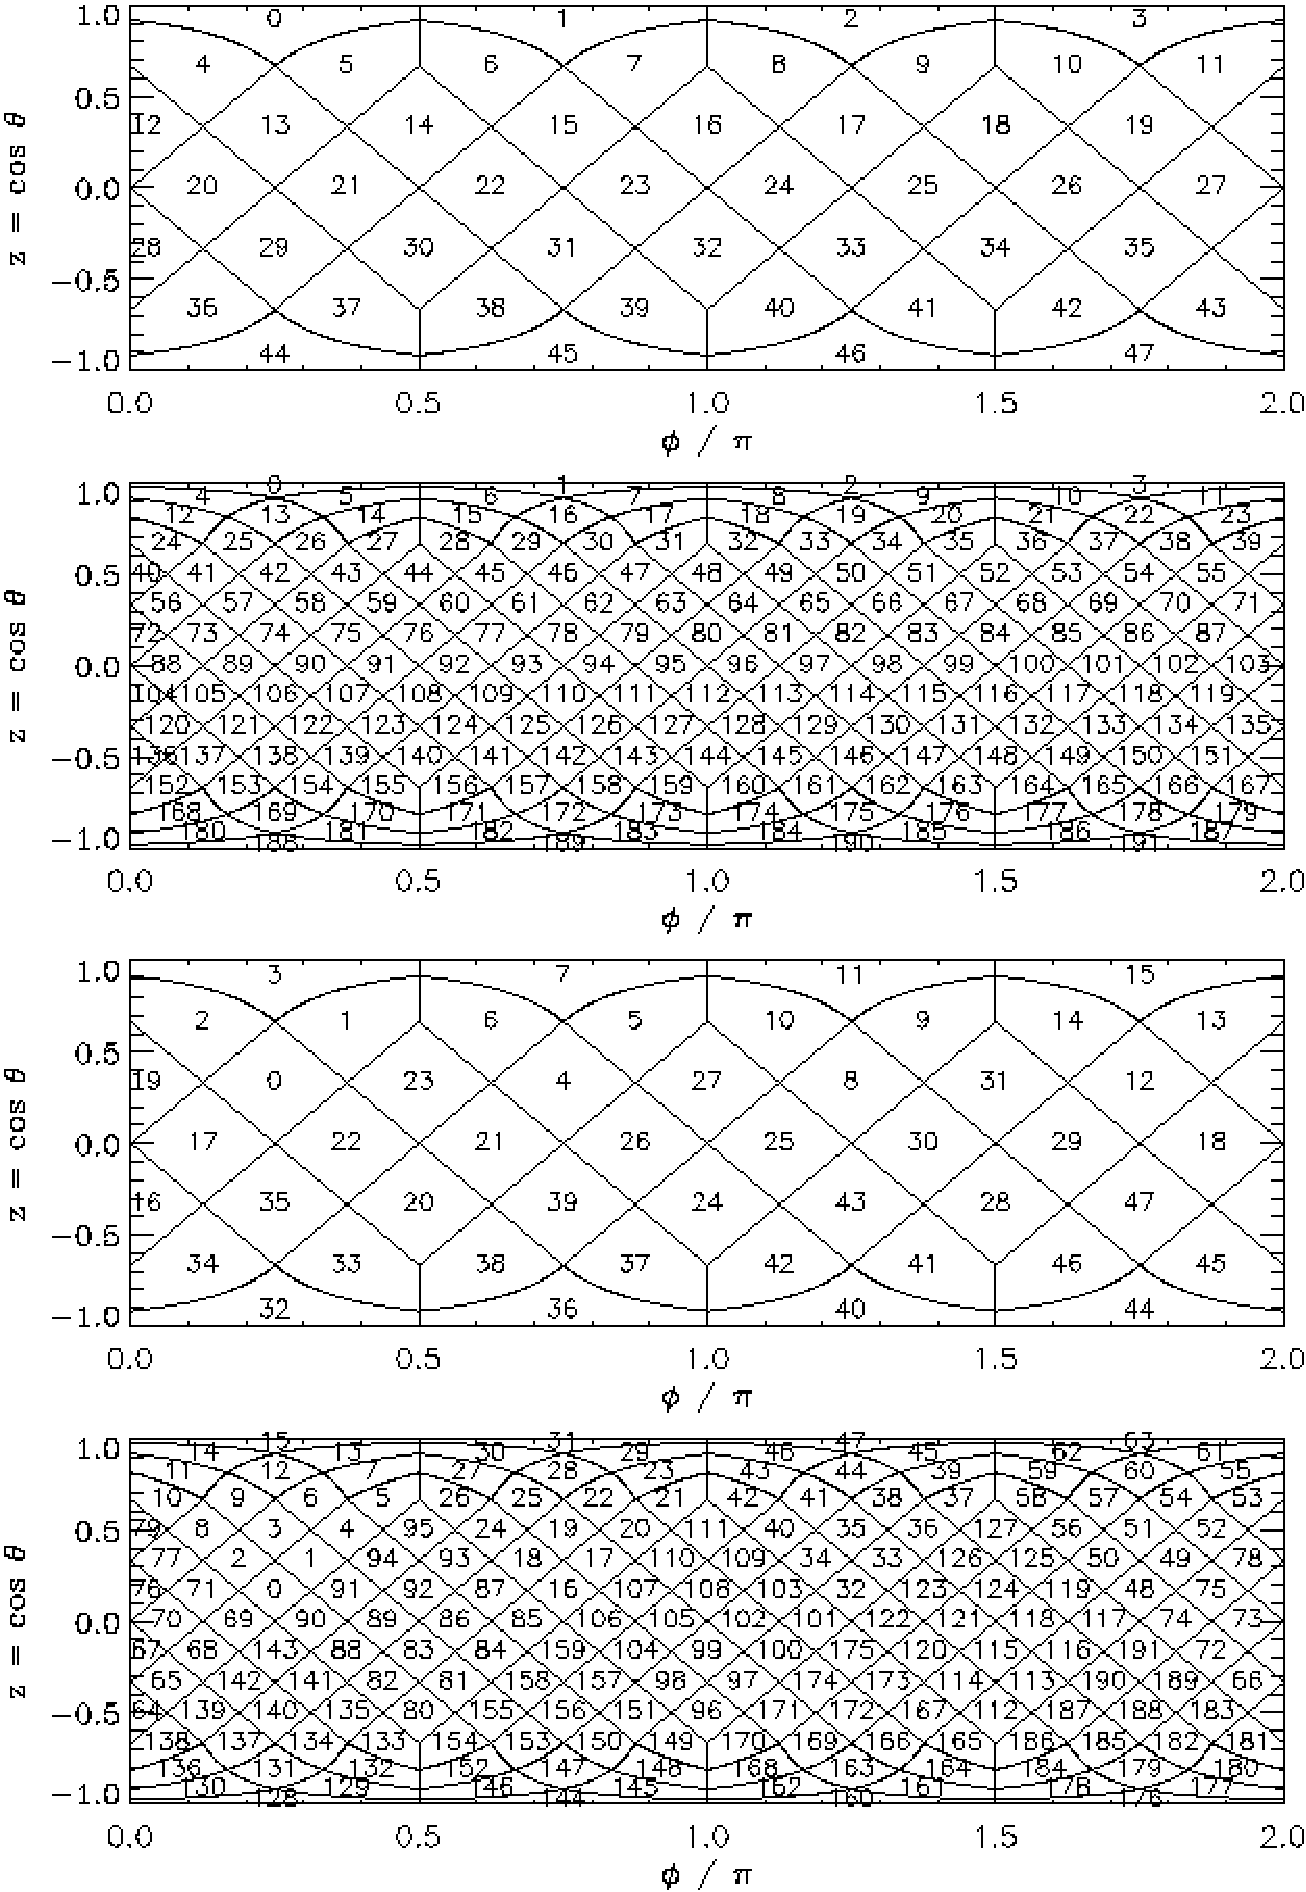
\includegraphics[height=10.5cm]{images/healpix2d.pdf}}
\caption[Cylindrical projection]%
{\label{fig:healpix_numbering}%
Cylindrical projection of the HEALPix division of a
sphere and two natural pixel numbering schemes (RING and NESTED). 
Both numbering schemes map the two dimensional 
distribution
of discrete area elements on a sphere into the one dimensional, 
integer pixel number array.
}
\end{center}
\end{figure}
\subsection{Rank-1 POVMs implementation}
We have already discussed how every qubit POVM can be written as a coarse graining of rank-1 projectors \cite{barrett2002}, such that the protocol implementation can restrict without any loss in generality to POVMs proportional to rank-1 projectors. 

Even if the final goal is to build POVMs to test how the classical protocol converges with the quantum theory for any random state and measurement, we will also discuss some general rank-1 POVMs with interesting properties, for example, 
\begin{enumerate}
    \item The measure needed in the eavesdropping  of the BB84 protocol \cite{nielsen2000}
\begin{equation}\label{eq:cross-povm}
    \mathbb{P}_4 = \{\frac{1}{2}\ket{0}\bra{0}, \frac{1}{2}\ket{1}\bra{1}, \frac{1}{2}\ket{+}\bra{+}, \frac{1}{2}\ket{-}\bra{-} \}
\end{equation}
    \item The Trine-POVM, consisting of POVM elements uniformly distributed on an equatorial plane of the Bloch sphere, with $\mathbb{P}_3=\{E_1, E_2, E_3\}$ and $E_k=\frac{2}{3}\ket{\Psi_{k}}\bra{\Psi_{k}}$, where
\begin{equation}\label{eq:trine-povm}
\begin{split}
\ket{\Psi_1}&=\ket{0}\\
\ket{\Psi_2}&=\frac{1}{2}\ket{0} + \frac{\sqrt{3}}{2} \ket{1}\\ 
\ket{\Psi_3}&=\frac{1}{2}\ket{0} - \frac{\sqrt{3}}{2} \ket{1}
\end{split}
\end{equation}
    \item The SIC-POVMs, a well-known family of symmetric informationally complete positive operator-valued measures, which are proven to be very relevant in quantum state tomography and quantum cryptography fields among others \cite{renes2004}. The simplest SIC-POVM is the one with states the vertices of a regular tetrahedron in the Bloch sphere, see Figure \ref{fig:sic_povm}, with $\mathbb{P}_4=\{E_1, E_2, E_3, E_4\}$ and $E_k=\frac{1}{2}\ket{\Psi_{k}}\bra{\Psi_{k}}$, where
\begin{equation}\label{eq:sic-povm}
\begin{split}
\ket{\Psi_1}&=\ket{0}\\ 
\ket{\Psi_2}&=\frac{1}{\sqrt{3}}\ket{0} + \sqrt{\frac{2}{3}} \ket{1}\\
\ket{\Psi_3}&=\frac{1}{\sqrt{3}}\ket{0} + \sqrt{\frac{2}{3}} \ e^{i\frac{2\pi}{3}} \ket{1}\\ 
\ket{\Psi_4}&=\frac{1}{\sqrt{3}}\ket{0} + \sqrt{\frac{2}{3}}\ e^{i\frac{4\pi}{3}} \ket{1}
\end{split}
\end{equation}
\end{enumerate}

The strategies to build the rank-1 POVMs and perform the measurement are different in the classical simulation protocol and in the quantum circuit model, as we will see later, so next sections will describe the methodologies applied for each case.

\begin{figure}[!ht]
\begin{center}
\centerline{\includesvg[height=4cm]{images/sic_povm.svg}}
\caption[SIC-POVM as tetrahedron in Bloch sphere]%
{\label{fig:sic_povm}%
In the Bloch sphere representation of a qubit, the states of a SIC-POVM form a regular tetrahedron with vertices $\ket{\Psi_1}=\ket{0}$, $\ket{\Psi_2}=1/{\sqrt{3}}\ket{0} + \sqrt{2/3} \ket{1}$, $\ket{\Psi_3}=1/{\sqrt{3}}\ket{0} + \sqrt{2/3} \ e^{i\frac{2\pi}{3}} \ket{1}$ and $\ket{\Psi_4}=1/{\sqrt{3}}\ket{0} + \sqrt{2/3}\ e^{i\frac{4\pi}{3}} \ket{1}$.}
\end{center}
\end{figure}

\subsubsection{Measurement in classical simulation protocols}\label{section:povm_generation}
As described by Sent\'is et al.\ \cite{sentis2013}, the conditions under which a set of $N$ arbitrary rank-1 operators $\{E_{k}\}$ comprises a qubit POVM such that $\sum_{k=1}^{N} a_{k} E_{k} = \mathbb{1}$, can be equivalently written in a system of four linear equations
\begin{equation}
    \sum_{k=1}^{N} a_{k} = 2
\end{equation}
\begin{equation}
    \sum_{k=1}^{N} a_{k} \vec{y}_{k} = \vec{0}
\end{equation}
where $\vec{y}_{k} \in \mathbb{R}^3$ are the Bloch vectors corresponding to the qubit pure states $\ket{v_{k}}$, such that $E_k = \ket{v_k}\bra{v_k}$. The existence of the set $\{a_{k}\}$ has a direct translation into a linear programming feasibility problem we would have to solve computationally.

As an example, to build a random POVM set of $N=4$ elements, we could apply the following procedure:
\begin{enumerate}
\item Assign two rank-1 operators as projective measurement elements $E_i = \ket{v_i}\bra{v_i}$ with unknown weights $\{a_i\} \text{, where}\ i=1,2$.
\item Apply the closure relation such that the third rank-1 operator is $E_3 = \mathbb{1} - \sum_{i=1}^{2}E_i$. Note that this will not be necessarily a rank-1 operator.
\item Diagonalize $E_3$ to obtain the relevant qubit states as eigenvectors $\ket{v_3}$ and $\ket{v_4}$.
\item Convert all qubit states $\ket{v_i}$ to Bloch vectors $\vec{y}_i \text{, where } i=1,2,...4$.
\item Solve the linear programming feasibility problem
\begin{equation*}
\begin{array}{ll@{}ll}
\text{find}  & x = \{a_1, a_2,\dots,a_N\} &\\
\text{subject to}& Ax = b\ \text{where column} \ A_{*k} = (\vec{y}_k, 1),\ \text{and}\ b = (\vec{0}, 2) \\
                 & x \geq 0 
\end{array}
\end{equation*}
\end{enumerate}

Provided the optimization problem is feasible, we obtain the weights $\{a_k\}$ and compute the rank-1 operators $E_k = \ket{v_k}\bra{v_k}$ which conform the POVM set elements $\{B_k\}$ such that $B_k=a_k E_k$. Then we can use Equation (\ref{eq:rank1_povm}) to perform the following assignment
\begin{equation}
    p_k = \frac{a_k}{2}
\end{equation}
\begin{equation}
    \ket{\vec{y}_k}\bra{\vec{y}_k} = E_k
\end{equation}
which will implement the POVMs in the form required by the classical simulation protocols, i.e. $B_{k} = 2p_{k}\ket{\vec{y}_{k}}\bra{\vec{y}_{k}}$.

\subsubsection{Measurement in quantum circuit model}\label{section:neumark}
To compare the probability distributions obtained from classical protocols with those from quantum simulators or noisy quantum computers, we must develop a technique for encoding positive operator-valued measures in a quantum circuit model. For a POVM of $N$ elements, such technique requires to create a $N\times N$ unitary matrix $U$ representing the measurement process.

Neumark's theorem \cite{neumark1940} asserts that one can extend the Hilbert space of states $\mathcal{H}$ in which rank-1 POVM elements 
\begin{equation}\label{eq:neumark_povm}
B_k = \ket{v_{k}} \bra{v_{k}},\ \text{where}\ \sum_{k=1}^{N} B_{k} = \mathbb{1}
\end{equation}
 are defined, in such a way that there exists in the extended space $\mathcal{K}$ a set of orthogonal projectors $\Pi_{k}$ such that $B_k$
 is the result of projecting $\Pi_{k}$ from $\mathcal{K}$ into $\mathcal{H}$. Following Peres \cite{peres1995}, we can add $N-2$ extra dimensions to $\mathcal{H}$ by introducing unit vectors $\ket{u_{k}}$ orthogonal to each other and to all $\ket{v_{k}}$ in Equation (\ref{eq:neumark_povm}). Then we can build a complete orthonormal basis $\ket{w_{k}}$ in the enlarged space $\mathcal{K}$ such that
\begin{equation}
\ket{w_{k}} := \ket{v_{k}} + \sum_{s=3}^{N} c_{k s} \ket{u_{k}}
\end{equation}
\begin{equation}\label{eq:neumark_orthonormal}
\bra{w_{j}} \ket{w_{k}} := \bra{v_{j}} \ket{v_{k}} + \sum_{s=3}^{N} c_{j s}^{\star} c_{k s} = \delta_{j k}
\end{equation}
where $c_{ks}$ are the complex coefficients to be determined. Eqs. (\ref{eq:neumark_povm}) and (\ref{eq:neumark_orthonormal}) can be rewritten in index notation as 
\begin{equation}\label{eq:neumark_closure_index}
\sum_{k=1}^{N}v_{k i}^{\star} v_{k j} = \delta_{ij}
\end{equation}
\begin{equation}\label{eq:neumark_orthonormal_index}
\sum_{i=1}^{2} v_{j i}^{\star} v_{k i} + \sum_{s=3}^{N} c_{j s}^{\star} c_{k s} = \delta_{j k}
\end{equation}
According to Equation (\ref{eq:neumark_orthonormal_index}) the following matrix $U$ is a unitary matrix which satisfies the closure property in Equation (\ref{eq:neumark_closure_index}) and encapsulates orthonormal states in the enlarged space $\mathcal{K}$ 
\begin{equation}
U = 
\begin{pmatrix}
v_{1 1} & v_{1 2} & c_{13} & \dots & c_{1 N} \\
v_{2 1} & v_{2 2} & c_{23} & \dots & c_{2 N} \\
\vdots & \vdots & \vdots & \vdots &  \vdots \\
v_{N1} & v_{N2} & c_{N3} & \dots & c_{NN}
\end{pmatrix}
\end{equation}
By computing the complex coefficients $c_{ks}$, we can then encode any rank-1 POVM measure into a unitary matrix $U$ which can be readily used within a quantum circuit model.
\subsection{Prepare-and-measure simulations}
In the following sections we will discuss the methods applied to implement the prepare-and-measure classical simulation protocols described in section \ref{section:protocols}.
\subsubsection{Classical transmission of one qubit}
So far we have described the methods available to generate random qubit states and random measurements proportional to rank-1 projectors. Once these are available, we should convert them to the corresponding elements in the Bloch sphere, i.e. to vectors $\vec{x}$, ${\vec{y}_k} \in \mathbb{R}^3$, as per protocol description (see section \ref{section:protocol_pm}). 

A qubit state in density matrix form $\rho$ can be easily be transformed into the dual Bloch vector $\vec{x}$ with components $\{x_k\}$ by applying the equation
\begin{equation}
    x_k = tr(\rho \cdot \sigma_k),\ \text{where}\ \vec{\sigma} = (\sigma_x, \sigma_y, \sigma_z)
\end{equation}
Similarly, the vector ${\vec{y}_k}$ associated to the POVM will be the Bloch vector corresponding to the rank-1 projector $ \ket{\vec{y}_k} \bra{\vec{y}_k}$, so the same procedure could be flawlessly applied.

For every random state and POVM, we will then sample the shared randomness $\vec{\lambda}_1$, $\vec{\lambda}_2 \in \mathbb{R}^3$ following a uniform distribution and will apply steps 1 to 4 in the protocol such that for every run we get the probability for each measurement outcome. Eq. (\ref{eq:prob_classic}) can then be computed by just using the probabilities outcomes as weights in a random choice whose outcome gets accumulated for each shared randomness run. The accumulated random choices will lead to the final probabilities which will be then compared against the ones obtained with either the theoretical probabilities as per Born's rule, or the probabilities obtained executing the associated quantum circuit in a quantum simulator (see section \ref{section:quantum_circuit}).

\subsubsection{Quantum circuit counterpart}\label{section:quantum_circuit}
Following Neumark's theorem described in section \ref{section:neumark}, we can now implement any POVM measure of $N$ elements in a quantum circuit by applying the $N\times N$ unitary matrix $U$ resulting from Neumark's theorem to an initial state made of the original qubit state we want to measure $\ket{\Psi}$, together with a set of $n-1$ ancillary qubits, a.k.a. \textit{ancillas}, in a zero state $\ket{0}$ such that $2^n \ge N$ (see Fig. \ref{fig:quantum_circuit}) 

\begin{figure}[!ht]
\centering
\def\myvdots{\ \vdots\ }
\begin{quantikz}
    \lstick[wires=4]{$\mathcal{H}^{\otimes n}$}
      && \lstick{$\ket{\Psi}$}  & \gate[4, nwires=3][2cm]{U} & \meter{} \\
      && \lstick{$\ket{0}$}  & & \meter{} & \rstick[wires=3]{$\mathcal{H}^{\otimes n-1}\ \text{ancilla qubits}$}\\
      && \lstick{\myvdots} & & \myvdots &\\
      && \lstick{$\ket{0}$}  & & \meter{} & 
\end{quantikz}
\caption{Quantum circuit implementing a POVM measure of $N$ outcomes following Neumark's extension theorem.}
\label{fig:quantum_circuit}
\end{figure}

As we can see in the diagram, we will obtain the different probabilities for each of the $N$ possible outcomes of the POVM, by adding an $n$ bit classical register to the circuit, which will then perform classical measures on the circuit's computational basis. Each outcome from a total set of $2^n$ possible outcomes of the classical register will therefore correspond to a POVM element measurement outcome. As an example, the measurement of a qubit state $\ket{\Psi}$ with a 4-element POVM as in Fig. \ref{fig:sic_povm}, will be encoded in a quantum circuit as a $4 \cross 4$ unitary matrix applied to the qubit state $\ket{\Psi}$ plus an ancillary qubit $\ket{0}$ such that all possible outcomes from the classical 2-bit register $\{00, 01, 10, 11\}$, will correspond to the measurement outcomes for each POVM element ($N=4$).

As we will show in section \ref{section:results}, these circuits will be implemented with Qiskit \cite{Qiskit}, IBM's open-source Quantum Computing SDK, and will be run using IBM's quantum processors to obtain the experimental probability distributions to be compared with the results from the classical simulations.

In order to translate the POVM's unitary matrices into universal quantum gates available in the underlying IBM's quantum processors, we could either follow Nielsen and Chuang's textbook \cite{nielsen2000}, and decompose the unitary into a sequence of two-level unitary gates, or rely on the Qiskit's transpiler, which translates any generic circuit into an optimized circuit using a backend's native gate set, allowing users to program for any quantum processor or processor architecture with minimal inputs. For the sake of simplicity we will follow on using Qiskit's transpiler. 

\subsection{Bell simulations}\label{section:methods_bell}
Most of the methods required to implement the classical simulation protocol described in Section \ref{section:protocol_bell} have already been addressed in the previous section. Hence, the underlying methodology for the generation of random states and measurements, dual Bloch vectors and shared randomness will be used without further discussion.

\subsubsection{Bell singlet state with projective measurements}

The classical protocol is applicable to Bell single states only, Alice is restricted to projective measurements with outcomes $a=\pm1$, and Bob can perform arbitrary POVMs, but we will restrict ourselves further with Bob performing arbitrary PVMs only, as per Toner and Bacon's original protocol \cite{toner2003}.

The expected joint probabilities will be computed for every possible combination of observables $A_{x}, B_{y}$, and outcomes $a_{x}, b_{y} = \pm1$. For every Bell singlet state and set of observables, we will then sample the shared randomness $\vec{\lambda}_1$, $\vec{\lambda}_2 \in \mathbb{R}^3$ following a uniform distribution and will apply steps 1 to 4 in the protocol such that for every run we get the probability for each measurement outcome. Eq. (\ref{eq:prob_classic_bell}) can then be computed by just using the probabilities outcomes as weights in a random choice whose outcome gets accumulated for each shared randomness run. The accumulated random choices will lead to the final probabilities which will be then compared against the ones obtained with Eq. (\ref{eq:prob_quantum_bell}).

\subsubsection{CHSH inequality}
In addition to the computation of joint probabilities, the expectation values for every duple of observables $\mathbb{E}[A_{x}, B_{y}]$ will also be calculated according to Eq. (\ref{eq:bell_expected_values}). That would allow us to use Eq. (\ref{eq:bell_inequality}) and try to prove through the classical protocol the breaking of Bell's inequality under a suitable set of observables by arguing that the $CHSH$ absolute value exceeds the classical upper bound that was deduced from the hypothesis of local hidden variable model, i.e.
\begin{equation}\label{eq:chsh_inequality}
|{CHSH}| \leq 2
\end{equation}